\documentclass [xcolor=svgnames, t] {beamer} 
\usepackage[utf8]{inputenc}
\usepackage{booktabs, comment} 
\usepackage[absolute, overlay]{textpos} 
\usepackage{pgfpages}
\usepackage[font=footnotesize]{caption}
\useoutertheme{infolines} 

\AtBeginSection[]{
  \begin{frame}
  \vfill
  \centering
  \begin{beamercolorbox}[sep=8pt,center,shadow=true,rounded=true]{title}
    \usebeamerfont{title}\insertsectionhead\par%
  \end{beamercolorbox}
  \vfill
  \end{frame}
}


%\definecolor{brownbrown}{RGB}{56, 28, 0}
%\definecolor{brownred}{RGB}{228, 0, 43}

%\setbeamercolor{title in head/foot}{bg=brownred, fg=brownbrown}
%\setbeamercolor{author in head/foot}{bg=myuniversity}
\setbeamertemplate{page number in head/foot}{}
\usepackage{csquotes}


\usepackage{amsmath}
\usepackage[makeroom]{cancel}


\usepackage{textpos}

\usepackage{tikz}

\usepackage{media9} 

\usetheme{Madrid}
%\definecolor{myuniversity}{RGB}{56, 28, 0}
%\usecolortheme[named=myuniversity]{structure}
\usepackage{tikz}



\title[Intro. e hist. fluidos]{Clase No.1: Introducci\'on}
\subtitle{Introducci\'on e historia de los fluidos}
\institute[]{Departamento de Ingenier\'ia Civil y Agr\'icola\\ Facultad de Ingenier\'ia  \\Universidad Nacional de Colombia - Sede Bogot\'a}
\titlegraphic{
\includegraphics[height=2.0cm]{escudoUnal.png}}
\author[LAM]{Luis Alejandro Morales \\ \href{https://lamhydro.github.io}{https://lamhydro.github.io}}

\date{\today}

\addtobeamertemplate{navigation symbols}{}{%
    \usebeamerfont{footline}%
    \usebeamercolor[fg]{footline}%
    \hspace{1em}%
    \insertframenumber/\inserttotalframenumber
}

\begin{document}
\begin{frame}
\maketitle
\end{frame}


%%%%%%%%%%%%%%%%%%%%%%%%%%%%
\logo{\vspace{-0.2cm}
\includegraphics[height=0.8cm]{escudoUnal.png}~%
}
%%%%%%%%%%%%%%%%%%%%%%%%%%



\begin{frame}
\frametitle{Table of Contents}
\tableofcontents
\end{frame}


\section{Introducci\'on}
\begin{frame}{Que es la mec\'anica de fluidos}
\begin{exampleblock}{}
La mec\'anica de fluidos es la ciencia que hace parte de la mecánica clásica la cual estudia los fluidos estáticos o en movimiento y su interacción con otros objetos o fluidos.
\end{exampleblock}
\end{frame}

\begin{frame}{Ramas de la mecánica de fluidos}
\begin{block}{Hidrodinámica}
Estudia fluidos en movimiento que pueden ser considerados incompresibles e.g. agua y gases a bajas velocidades.
\end{block}
\begin{figure}
\centering
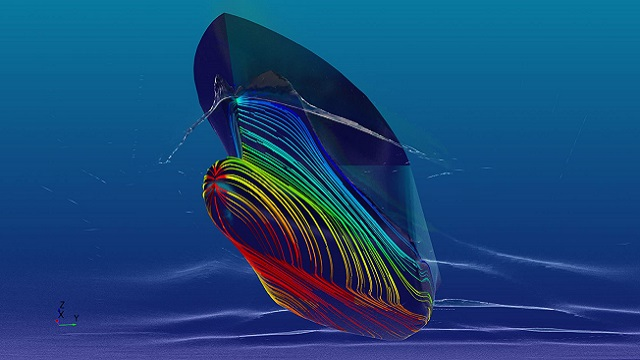
\includegraphics[width=0.33\textwidth]{hydro1}
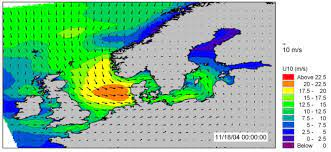
\includegraphics[width=0.33\textwidth]{hydro2}
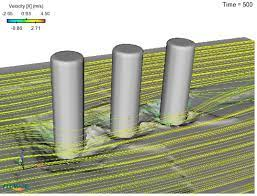
\includegraphics[width=0.33\textwidth]{hydro3}
\end{figure}
\end{frame}

\begin{frame}{Ramas de la mecánica de fluidos}
\begin{block}{Hidráulica}
Estudia el movimiento de líquidos en tuberías y canales abiertos (e.g. Rios).
\end{block}
\begin{figure}
\centering
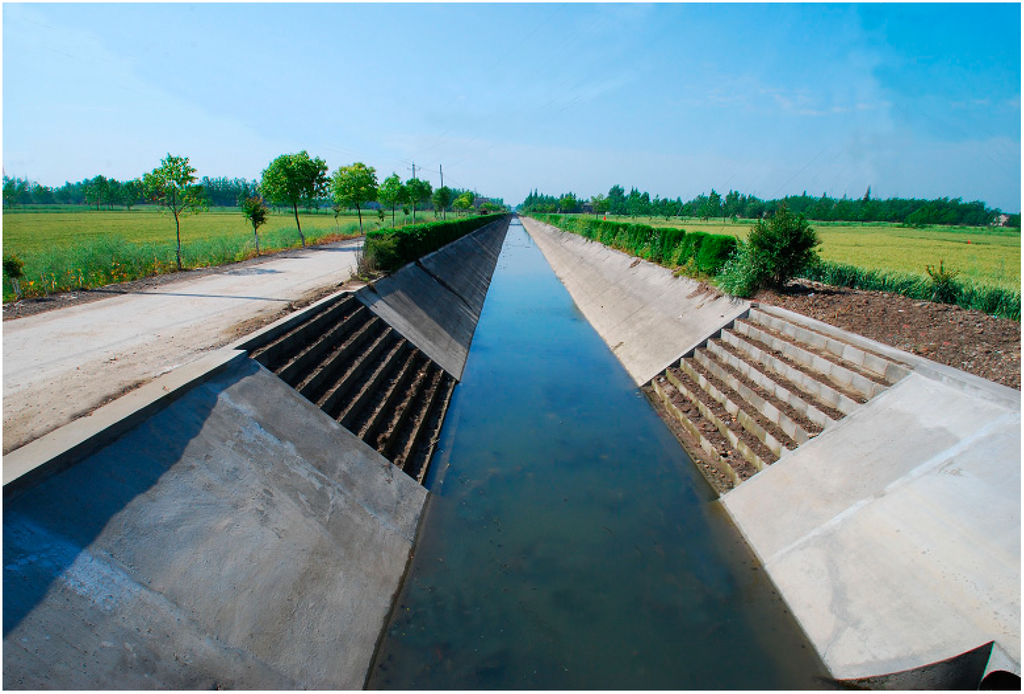
\includegraphics[width=0.45\textwidth]{hydra1}
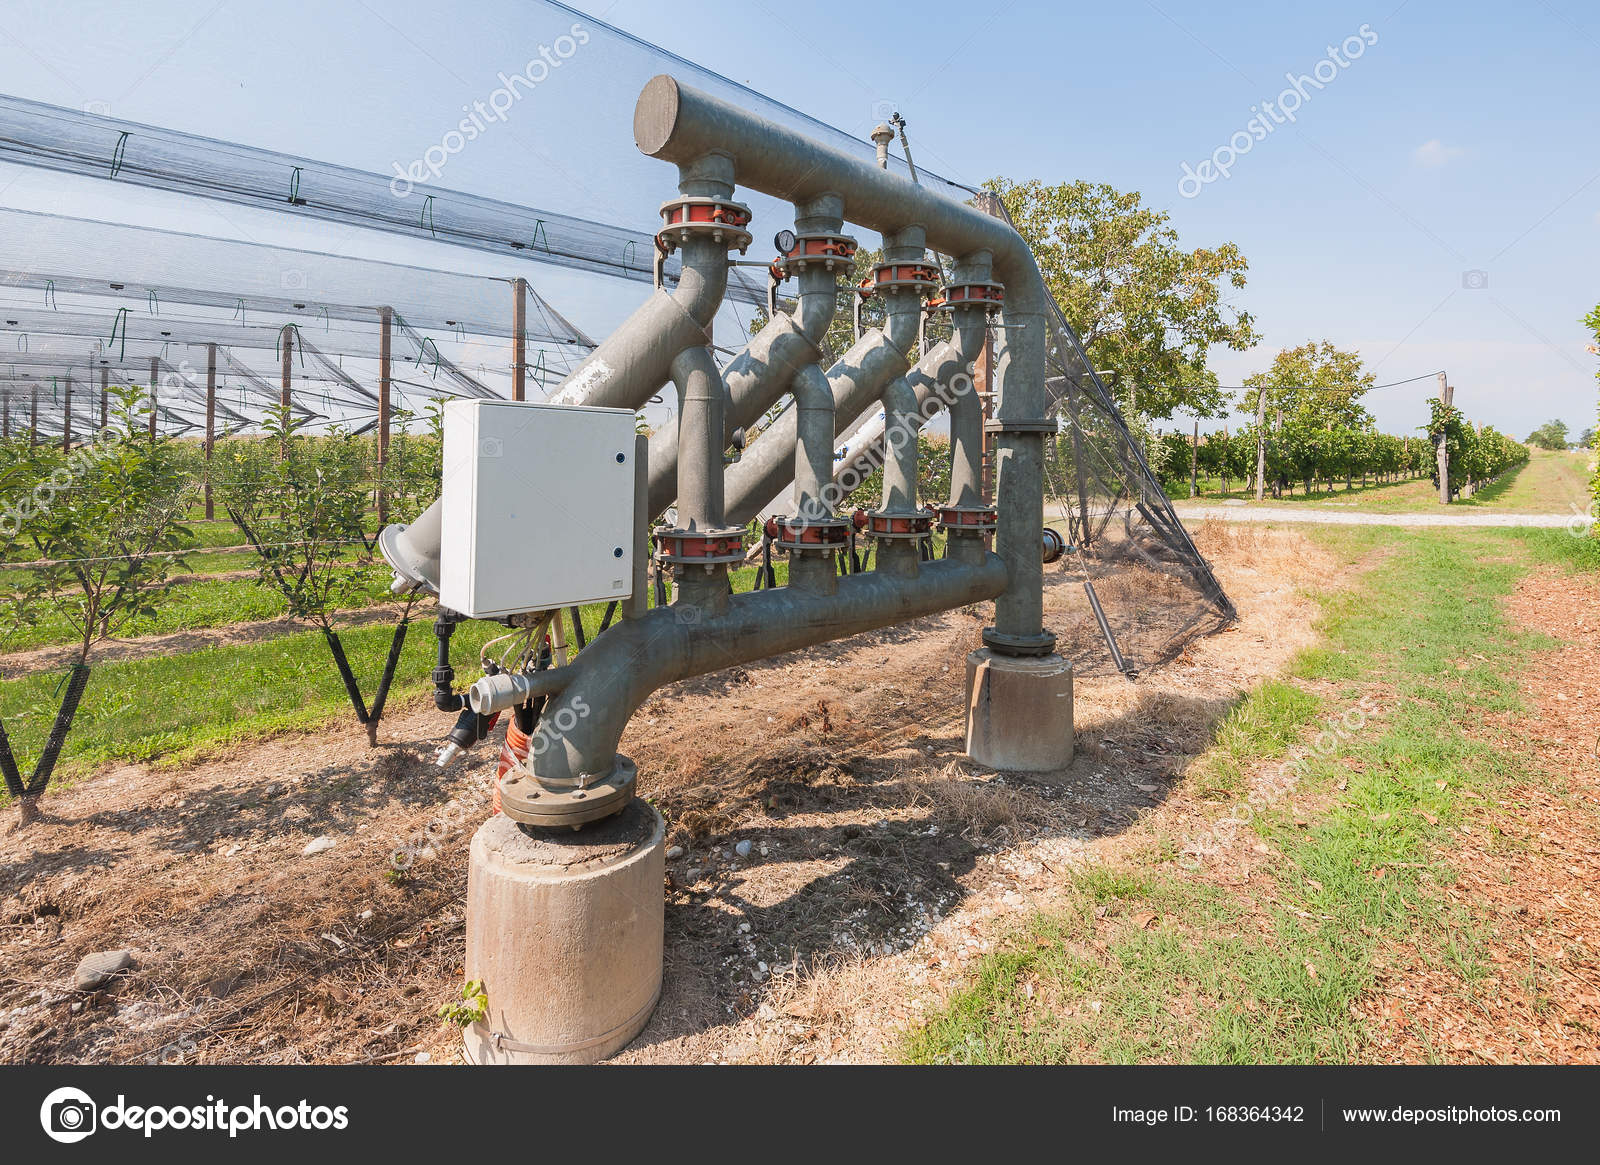
\includegraphics[width=0.45\textwidth]{hydra2}
\end{figure}
\end{frame}

\begin{frame}{Ramas de la mecánica de fluidos}
\begin{block}{Dinámica de gases}
Estudia el flujo de fluidos sometidos a cambios importantes de la densidad, e.g. flujo de gases a alta velocidad.
\end{block}
\begin{figure}
\centering
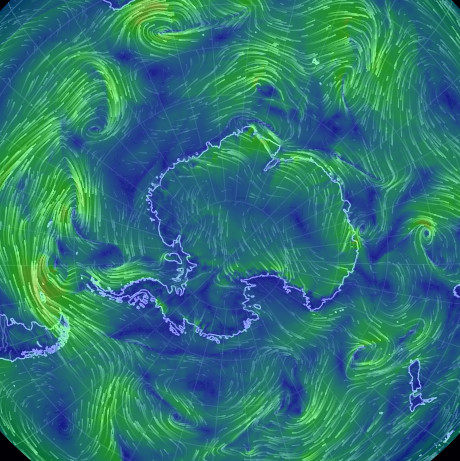
\includegraphics[width=0.45\textwidth]{gasd1}
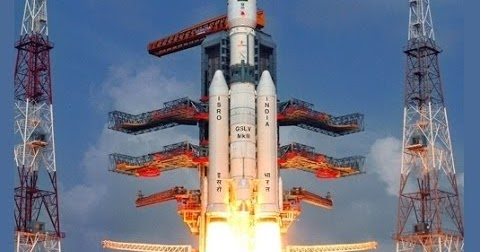
\includegraphics[width=0.45\textwidth]{gasd2}
\end{figure}
\end{frame}

\begin{frame}{Ramas de la mecánica de fluidos}
\begin{block}{Aerodinámica}
Estudio del movimiento de gases, principalmente aire, alrededor de objetos e.g. cabina de un avión, cohetes y automóviles.
\end{block}
\begin{figure}
\centering
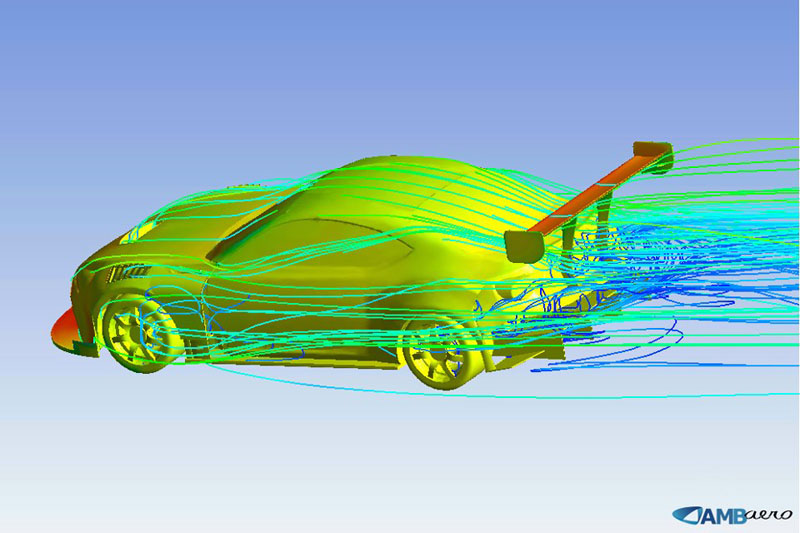
\includegraphics[width=0.45\textwidth]{aero1}
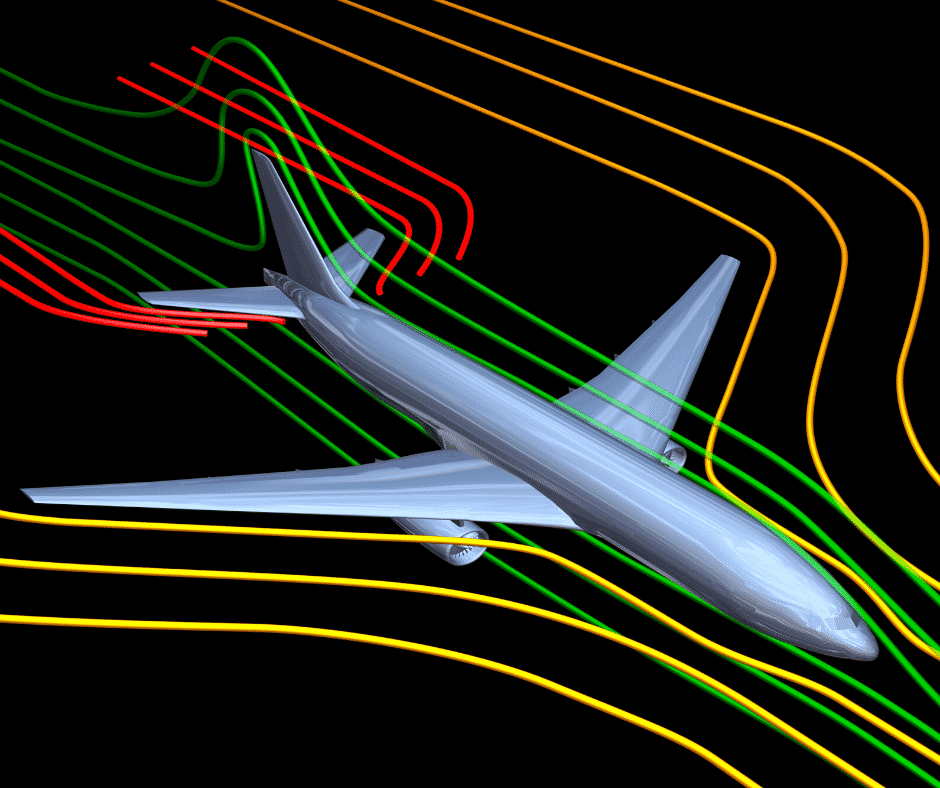
\includegraphics[width=0.45\textwidth]{aero2}
\end{figure}
\end{frame}

\begin{frame}{Estado de los fluidos}
De la física, la materia existe en cuatro diferentes estados:
\begin{itemize}
\item Solido
\item Liquido 
\item Gas
\item Plasma (fluido a altas temperaturas)
\end{itemize}
 
\begin{exampleblock}{Liquido vs solido}
La diferencia entre un liquido y un solido es en la habilidad de resistir esfuerzos que tienden a cambiar su forma. Por lo tanto, mientras un solido es capaz de resistir esfuerzos cuando se deforma, \textbf{un fluido se deforma continuamente y sin parar cuando se aplica un esfuerzo} sin importar su magnitud. 
\end{exampleblock}
\end{frame}

\begin{frame}{¿Que es un fluido?}
\href{https://www.youtube.com/watch?v=G53gvVh230U}{\beamergotobutton{Link}}
%\includemedia[
%  width=0.6\linewidth,height=0.45\linewidth,
%  activate=pageopen,
%  flashvars={
%    modestbranding=1 % no YT logo in control bar
%   &autohide=1       % controlbar autohide
%   &showinfo=0       % no title and other info before start
%  }
%]{}{https://www.youtube.com/watch?v=G53gvVh230U}   % Flash file
\end{frame}

\begin{frame}{Deformaciones en un fluido}
%Sin consideramos la goma solida de la Figura~\ref{f1} la cual esta fija a una base y a la cual se le aplica una fuerza $F$ paralela a la base, la goma se deforma y su angulo de deformacion ($\alpha$), denominado \texttt{resistencia al esfuerzo} o \texttt{desplazamiento angular}, es proporcional a $F$. La fuerza actuante contraria a $F$ debido a la friccion entre la plaza superior y la goma, es igual $F=\tau A$ donde $\tau$ es el esfuerzo cortante y $A$ es el area de contacto entre ambas superficies. Si en lugar de la goma tuvieramos un liquido, las capas mas cercanas a la placa superior se moverian continuamente, sin importar la magnitud de la fuerza, y la velocidad decreceria con la profundidad.
\centering
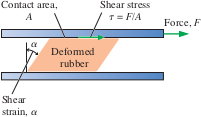
\includegraphics[width=6cm]{fig1}

\begin{itemize}
\item $F$: Fuerza paralela a la base
\item $\alpha$: \textbf{resistencia al esfuerzo} o \textbf{desplazamiento angular}. $\alpha$ $\propto$ $F$
\item $F_f =\tau A$. Fuerza de fricci\'on, donde $\tau$ es el esfuerzo cortante y $A$ es el área de contacto
\end{itemize}
\begin{exampleblock}{}
Si en lugar de la goma tuviéramos un liquido, las capas mas cercanas a la placa superior se moverían continuamente, sin importar la magnitud de la fuerza, y la velocidad decrecería con la profundidad.
\end{exampleblock}
\end{frame}

%De la estatica de cuerpos podemos definir:
%\begin{exampleblock}
%Estres se define como la fuerza por unidad de area y se calcula como fuerza $F$ divida por el area $A$ sobre la cual actua la fuerza. Al descomponer la fuerza actuante, la fuerza normal dividad por el area es el estres normal y la componente tangencial por unidad de area es el esfuerzo cortante. Por ejemplo en un fluido en reposo (esfuerzo cortante igual a cero), el esfuerzo normal es la presion.
%\end{exampleblock} 


\begin{frame}{Líquidos vs gases}
\vspace{-0.5cm}
\begin{exampleblock}{}
Líquidos y gases (o vapores) se diferencian en que al tener un liquido en un contenedor, el volumen del liquido permanece constante formando una superficie libre porque la fuerza de cohesión entre las moléculas es alta y las moléculas están cerca. En contraste, en un gas las moléculas se mueven aleatoriamente y están mas alejadas y tienden a ocupar todo el volumen del contenedor debido a la débil fuerza cohesiva de sus moléculas. Fluidos como el asfalto o lodos se comportan como solidos y líquidos dependiente de la magnitud de los esfuerzos aplicados. 
\end{exampleblock}
\centering
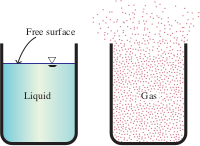
\includegraphics[width=5.5cm]{liqGas}
\end{frame}


\begin{frame}{Fluido como un continuo}
\centering
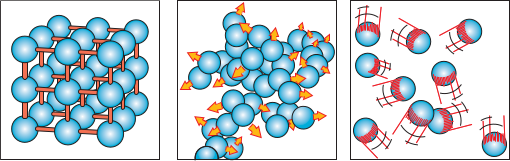
\includegraphics[width=5.5cm]{conti}
\begin{exampleblock}{}
\begin{itemize}
\item El diámetro de las moléculas es pequeño comparado con el espaciamiento entre ellas
\item Las moléculas se mueven libremente
\item A nivel microscópico, la densidad cambia constantemente. Estos cambios son despreciables para volúmenes relativamente grandes 
\item Sin embargo, la densidad $rho$ cambia suavemente con el espacio y con el tiempo en aplicaciones reales: a esto se le llama \emph{continuo}. Lo contrario seria un análisis molecular
\item Calculo diferencial es utilizado para analizar estas substancias
\end{itemize}
\end{exampleblock}
\end{frame}

\section{Historia de la mec\'anica de fluidos}
\begin{frame}{Historia de la mec\'anica de fluidos}
\begin{exampleblock}{}
\begin{itemize}
\item Uno de los grandes problemas de la humanidad ha sido el suministro de agua para uso domestico e irrigación.
\item Las sociedades prehistóricas que perduraron fueron también aquellas que invirtieron en la construcción de sistemas de distribución de agua.
\end{itemize}
\end{exampleblock}
\end{frame}

\begin{frame}{Prehistoria}
\vspace{-0.5cm}
\begin{columns}
\column{0.5\textwidth}
Los acueductos del Imperio Romano (312 B.C.)\\
\centering
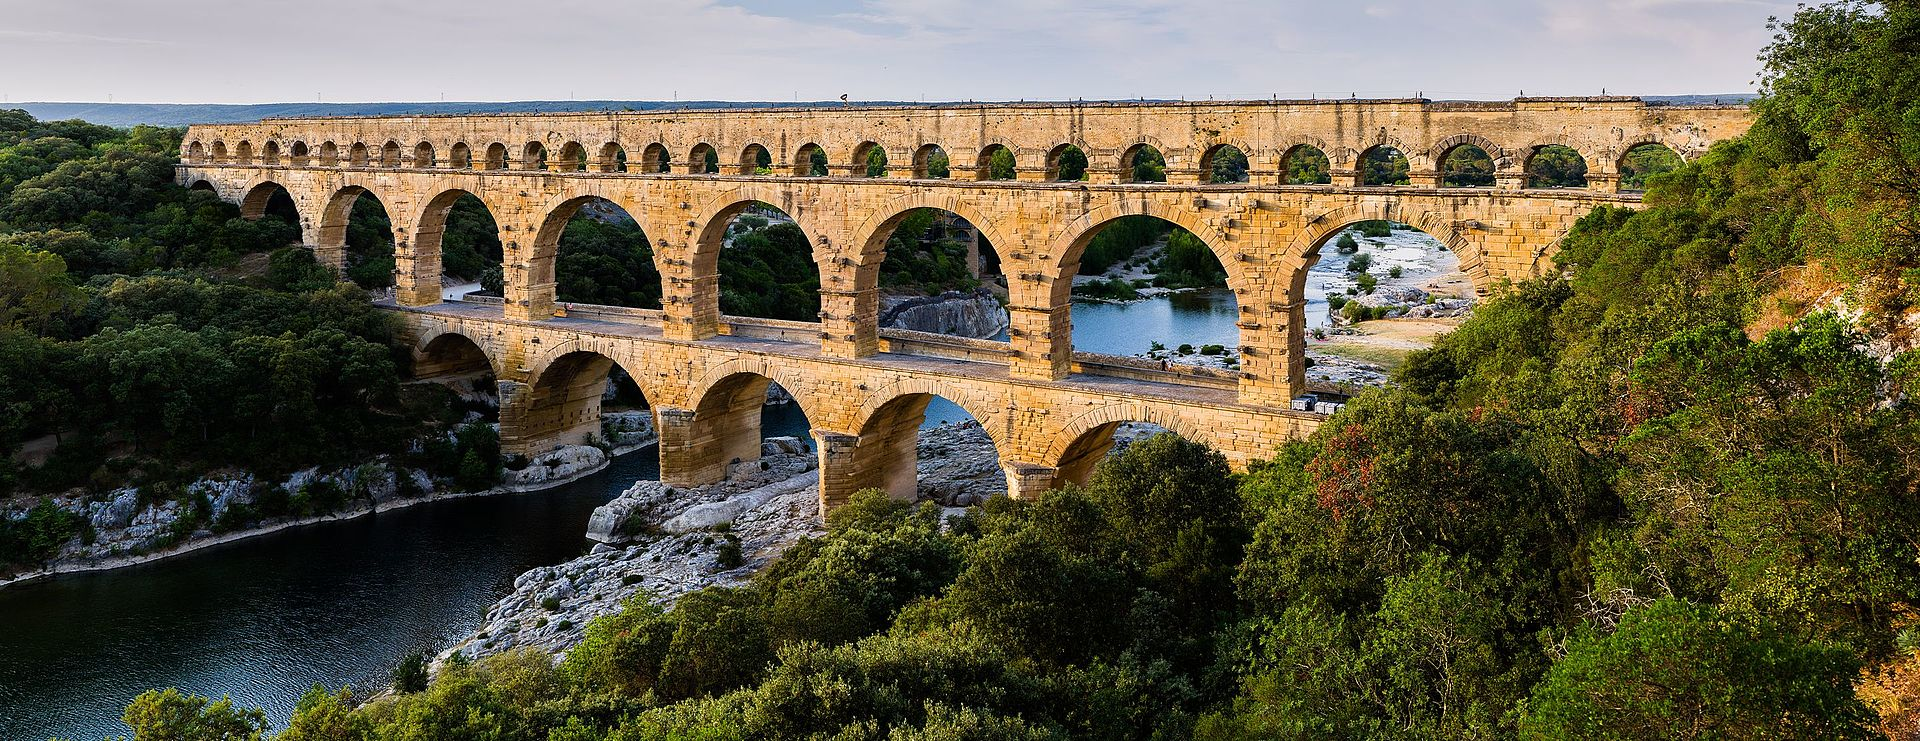
\includegraphics[width=0.55\textwidth]{romans}
\centering
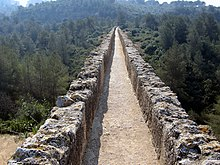
\includegraphics[width=0.55\textwidth]{romans2}
\column{0.5\textwidth}
45 km de tubería en arcilla que transportaban agua a presión $>$1.5 Mpa (180 m cabeza de agua) ciudad Helenica de Pergamo, Turkey (283-133 B.C.) \\
\centering
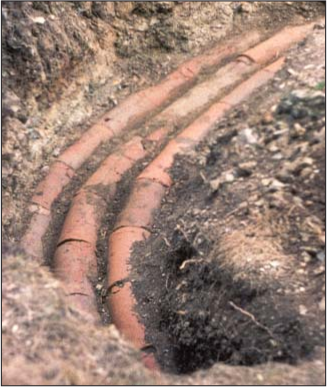
\includegraphics[width=0.5\textwidth]{pergamo}
\end{columns}
\begin{block}{Arquímedes}
El matemático Griego Arquímedes (285-212 B.C.) formulo y aplico el principio de flotación para saber la cantidad de oro en la corona del Rey Hieron de Siracusa.
\end{block}
\end{frame}

\begin{frame}{Edad media}
\begin{columns}
\column{0.5\textwidth}
Bombas de pistón fueron construidas para extraer el agua de las minas\\
\centering
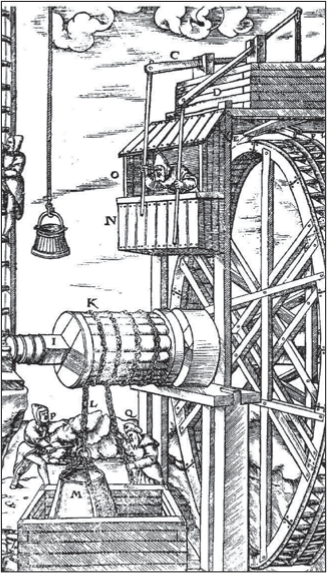
\includegraphics[width=0.6\textwidth]{minas}
\column{0.5\textwidth}
Molinos de agua y de viento fueron desarrollados para moler granos y trabajar el hierro reemplazando la fuerza humana. Dio luego origen a la Revolución Industrial.\\
\centering
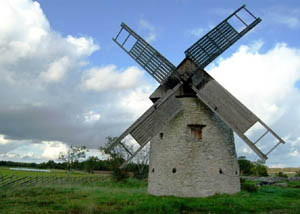
\includegraphics[width=0.9\textwidth]{wind}
\end{columns}
\end{frame}

\begin{frame}{Renacimiento}
\begin{columns}
\column{0.8\textwidth}
\vspace{-0.5cm}
\begin{exampleblock}{}
\begin{itemize}
\item Importantes avances en la mecánica de fluidos gracias al desarrollo del Método Científico
\item Simon Stevin (1548–1617), \emph{Galileo Galilei (1564–1642)}, Edme Mariotte (1620–1684), y Evangelista Torricelli (1608–1647) fueron los primero en aplicar el método al estudio de los fluidos para entender la distribución de presiones hidroestática. El matemático y filosofo \emph{Blaise Pascal (1623–1662)} mejoro e integro estos trabajos sobre hidroestatica.
\item Benedetto Castelli (1577–1644) fue el primero en publicar el principio de continuidad en fluidos.
\item \emph{Sir Isaac Newton (1643–1727)} aplic\'o las leyes de la mecánica a fluidos para explorar la inercia, la resistencia y la  viscosidad en fluidos.
\end{itemize}
\end{exampleblock}
\column{0.2\textwidth}
\vspace{-0.4cm}
\begin{center}
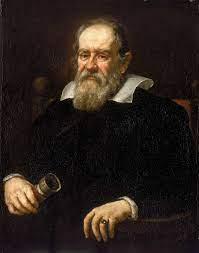
\includegraphics[width=0.7\textwidth]{gali}\\
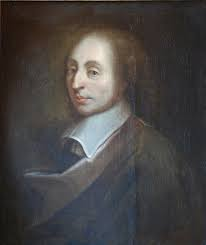
\includegraphics[width=0.7\textwidth]{pasca}\\
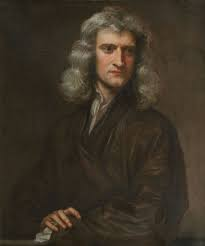
\includegraphics[width=0.7\textwidth]{new}
\end{center}
\end{columns}
\end{frame}

\begin{frame}{Renacimiento}
\begin{columns}
\column{0.8\textwidth}
\vspace{-0.4cm}
\begin{exampleblock}{}
\begin{itemize}
\item \emph{Daniel Bernoulli (1700–1782)} y \emph{Leonard Euler (1707–1783)}, basados en los desarrollos de Newton, definieron las ecuaciones de conservación de la energía y de momentum.
\item \emph{Hydrodynamica}, escrito por Bernoulli en 1738, es considerado el primer libro de mecánica de fluidos.
\item Jean d’Alembert (1717–1789) desarrollo una expresión diferencial de la continuidad basado en la idea de las componentes de la velocidad y la aceleración.
\item Debido a la dificultad de cuantificar propiedades de los fluidos, poco impacto tuvieron estos desarrollos en la ingeniería. 
\end{itemize}
\end{exampleblock}
\column{0.2\textwidth}
\vspace{-0.8cm}
\begin{center}
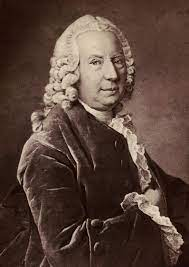
\includegraphics[width=0.8\textwidth]{berno}\\
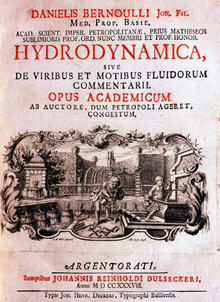
\includegraphics[width=0.8\textwidth]{hydrody}\\
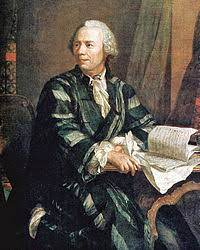
\includegraphics[width=0.8\textwidth]{euler}
\end{center}
\end{columns}
\end{frame}

\begin{frame}{Siglo XIX (Europa)}
\vspace{-0.4cm}
\begin{exampleblock}{}
\begin{itemize}
\item Se introduce C\'alculo en el pensum de las escuelas de ingeniería y esto genera grandes desarrollos durante este siglo:
\item \emph{Jean Poiseuille (1799–1869)} midió flujo en flujos capilares para diferentes fluidos
\item En Alemania, \emph{Gotthilf Hagen (1797–1884)} hizo experimentos para diferenciar flujo laminar y flujo turbulento en tuberías.
\end{itemize}
\end{exampleblock}
\begin{center}
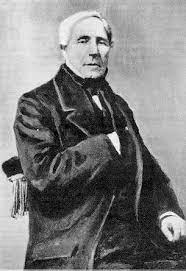
\includegraphics[width=0.26\textwidth]{poise}\hspace{2cm}
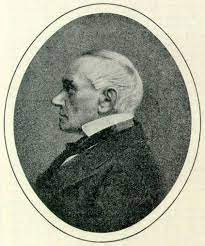
\includegraphics[width=0.26\textwidth]{hagen}
\end{center}
\end{frame}

\begin{frame}{Siglo XIX (Europa)}
\vspace{-0.4cm}
\begin{exampleblock}{}
\begin{itemize}
\item En Inglaterra, \emph{Lord Osborne Reynolds (1842–1912)} continuo el trabajo de Hagen y desarrollo el numero adimensional que lleva su nombre.
\item En paralelo, \emph{Louis Navier (1785–1836)} y \emph{George Stokes (1819–1903)} establecieron las ecuaciones del movimiento de los fluidos. Este ultimo incluyo la fricción.
\item \emph{William Froude (1810–1879)} demostró la importancia de la modelaci\'on física.
\end{itemize}
\end{exampleblock}
\begin{center}
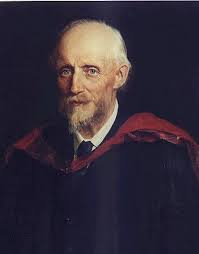
\includegraphics[width=0.2\textwidth]{reyn}
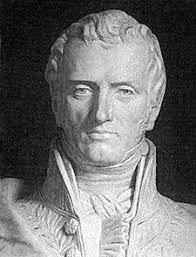
\includegraphics[width=0.2\textwidth]{navier}
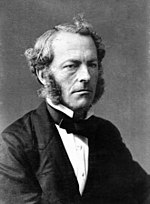
\includegraphics[width=0.2\textwidth]{stoke}
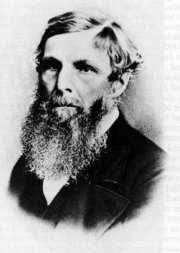
\includegraphics[width=0.2\textwidth]{froude}
\end{center}
\end{frame}


\begin{frame}{Finales del XIX (Estados Unidos)}
\vspace{-0.4cm}
\begin{exampleblock}{}
\begin{itemize}
\item \emph{James Francis (1815–1892)} y \emph{Lester Pelton (1829–1908)}, aplicando la teoría hasta ahora desarrollada, construyeron y comercializaron turbinas.
\item \emph{Clemens Herschel (1842–1930)} invento el \emph{tubo Venturi} para medir caudales de flujo.
\end{itemize}
\end{exampleblock}
\begin{center}
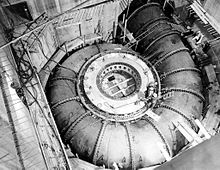
\includegraphics[width=0.3\textwidth]{franc}
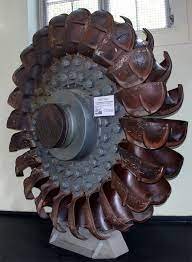
\includegraphics[width=0.3\textwidth]{pelton}
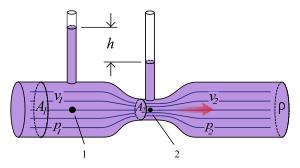
\includegraphics[width=0.3\textwidth]{ventu}
\end{center}
\end{frame}

\begin{frame}{Finales del XIX (Inglaterra)}
\vspace{-0.4cm}
\begin{exampleblock}{}
William Thomson, Lord Kelvin (1824–1907), William Strutt, Lord Rayleigh (1842–1919), and Sir Horace Lamb (1849–1934) fueron pioneros en investigar: análisis dimensional, flujo irrotacional, vortices, cavitaci\'on y olas. Exploraron las relaciones entre la mecánica de fluidos, la termodinámica y la transferencia de calor.
\end{exampleblock}
\end{frame}

\begin{frame}{Primera mitad del siglo XX}
\begin{columns}
\column{0.3\textwidth}
Los autodidactas \emph{hermanos Wright (1903)} inventaron el avión usando conceptos de la mecánica de fluidos y haciendo experimentos.\\
\centering
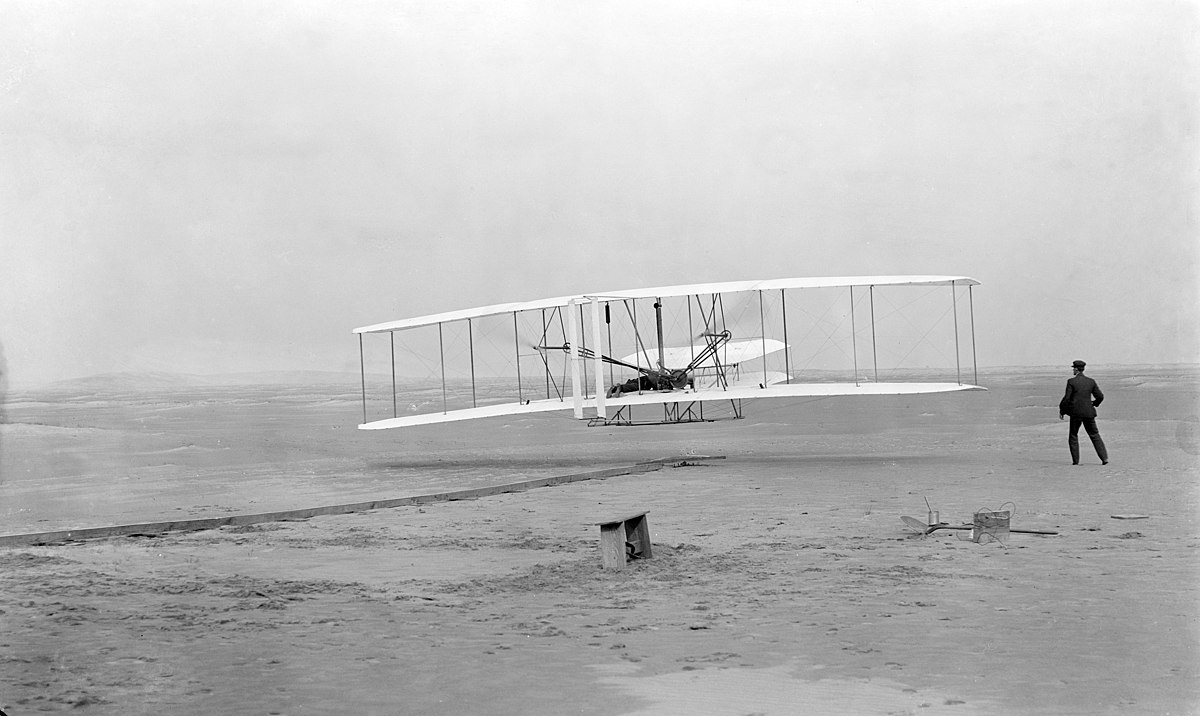
\includegraphics[width=1.1\textwidth]{wrig}
\column{0.7\textwidth}
\vspace{-1cm}
\begin{itemize}
\item El aleman \emph{Ludwig Prandtl (1875–1953)}, demostró que los fluidos pueden dividirse en dos partes: una capa delgada cerca a la pared en donde la fricción es importante llamada capa limite, y otro capa en donde la fricción es despreciable y las ecuaciones simplificadas de Euler y Bernoulli pueden aplicarse.
\item Con base en las teorías de Prandtl, Theodor von Kármán (1881–1963), Paul Blasius (1883–1970), Johann Nikuradse (1894–1979) y otros avanzaron en aplicaciones de la hidráulica y la aerodinámica.
\end{itemize}
\end{columns}
\end{frame}

\begin{frame}{Segunda mitad del siglo XX}
\vspace{-0.4cm}
\begin{exampleblock}{}
\begin{itemize}
\item Los a\~nos dorados de las aplicaciones de la mecánica de fluidos: grandes desarrollos en sectores de la aeronáutica, la industria química y los recursos hidráulicos.
\item Importantes investigaciones avanzaron con el invento del computados digital. Gracias a esto, fue posible trabajar en problemas complejos como la circulación global de la atmósfera y de los océanos, y la optimización en el diseño de turbinas.
\end{itemize}
\end{exampleblock}
\begin{center}
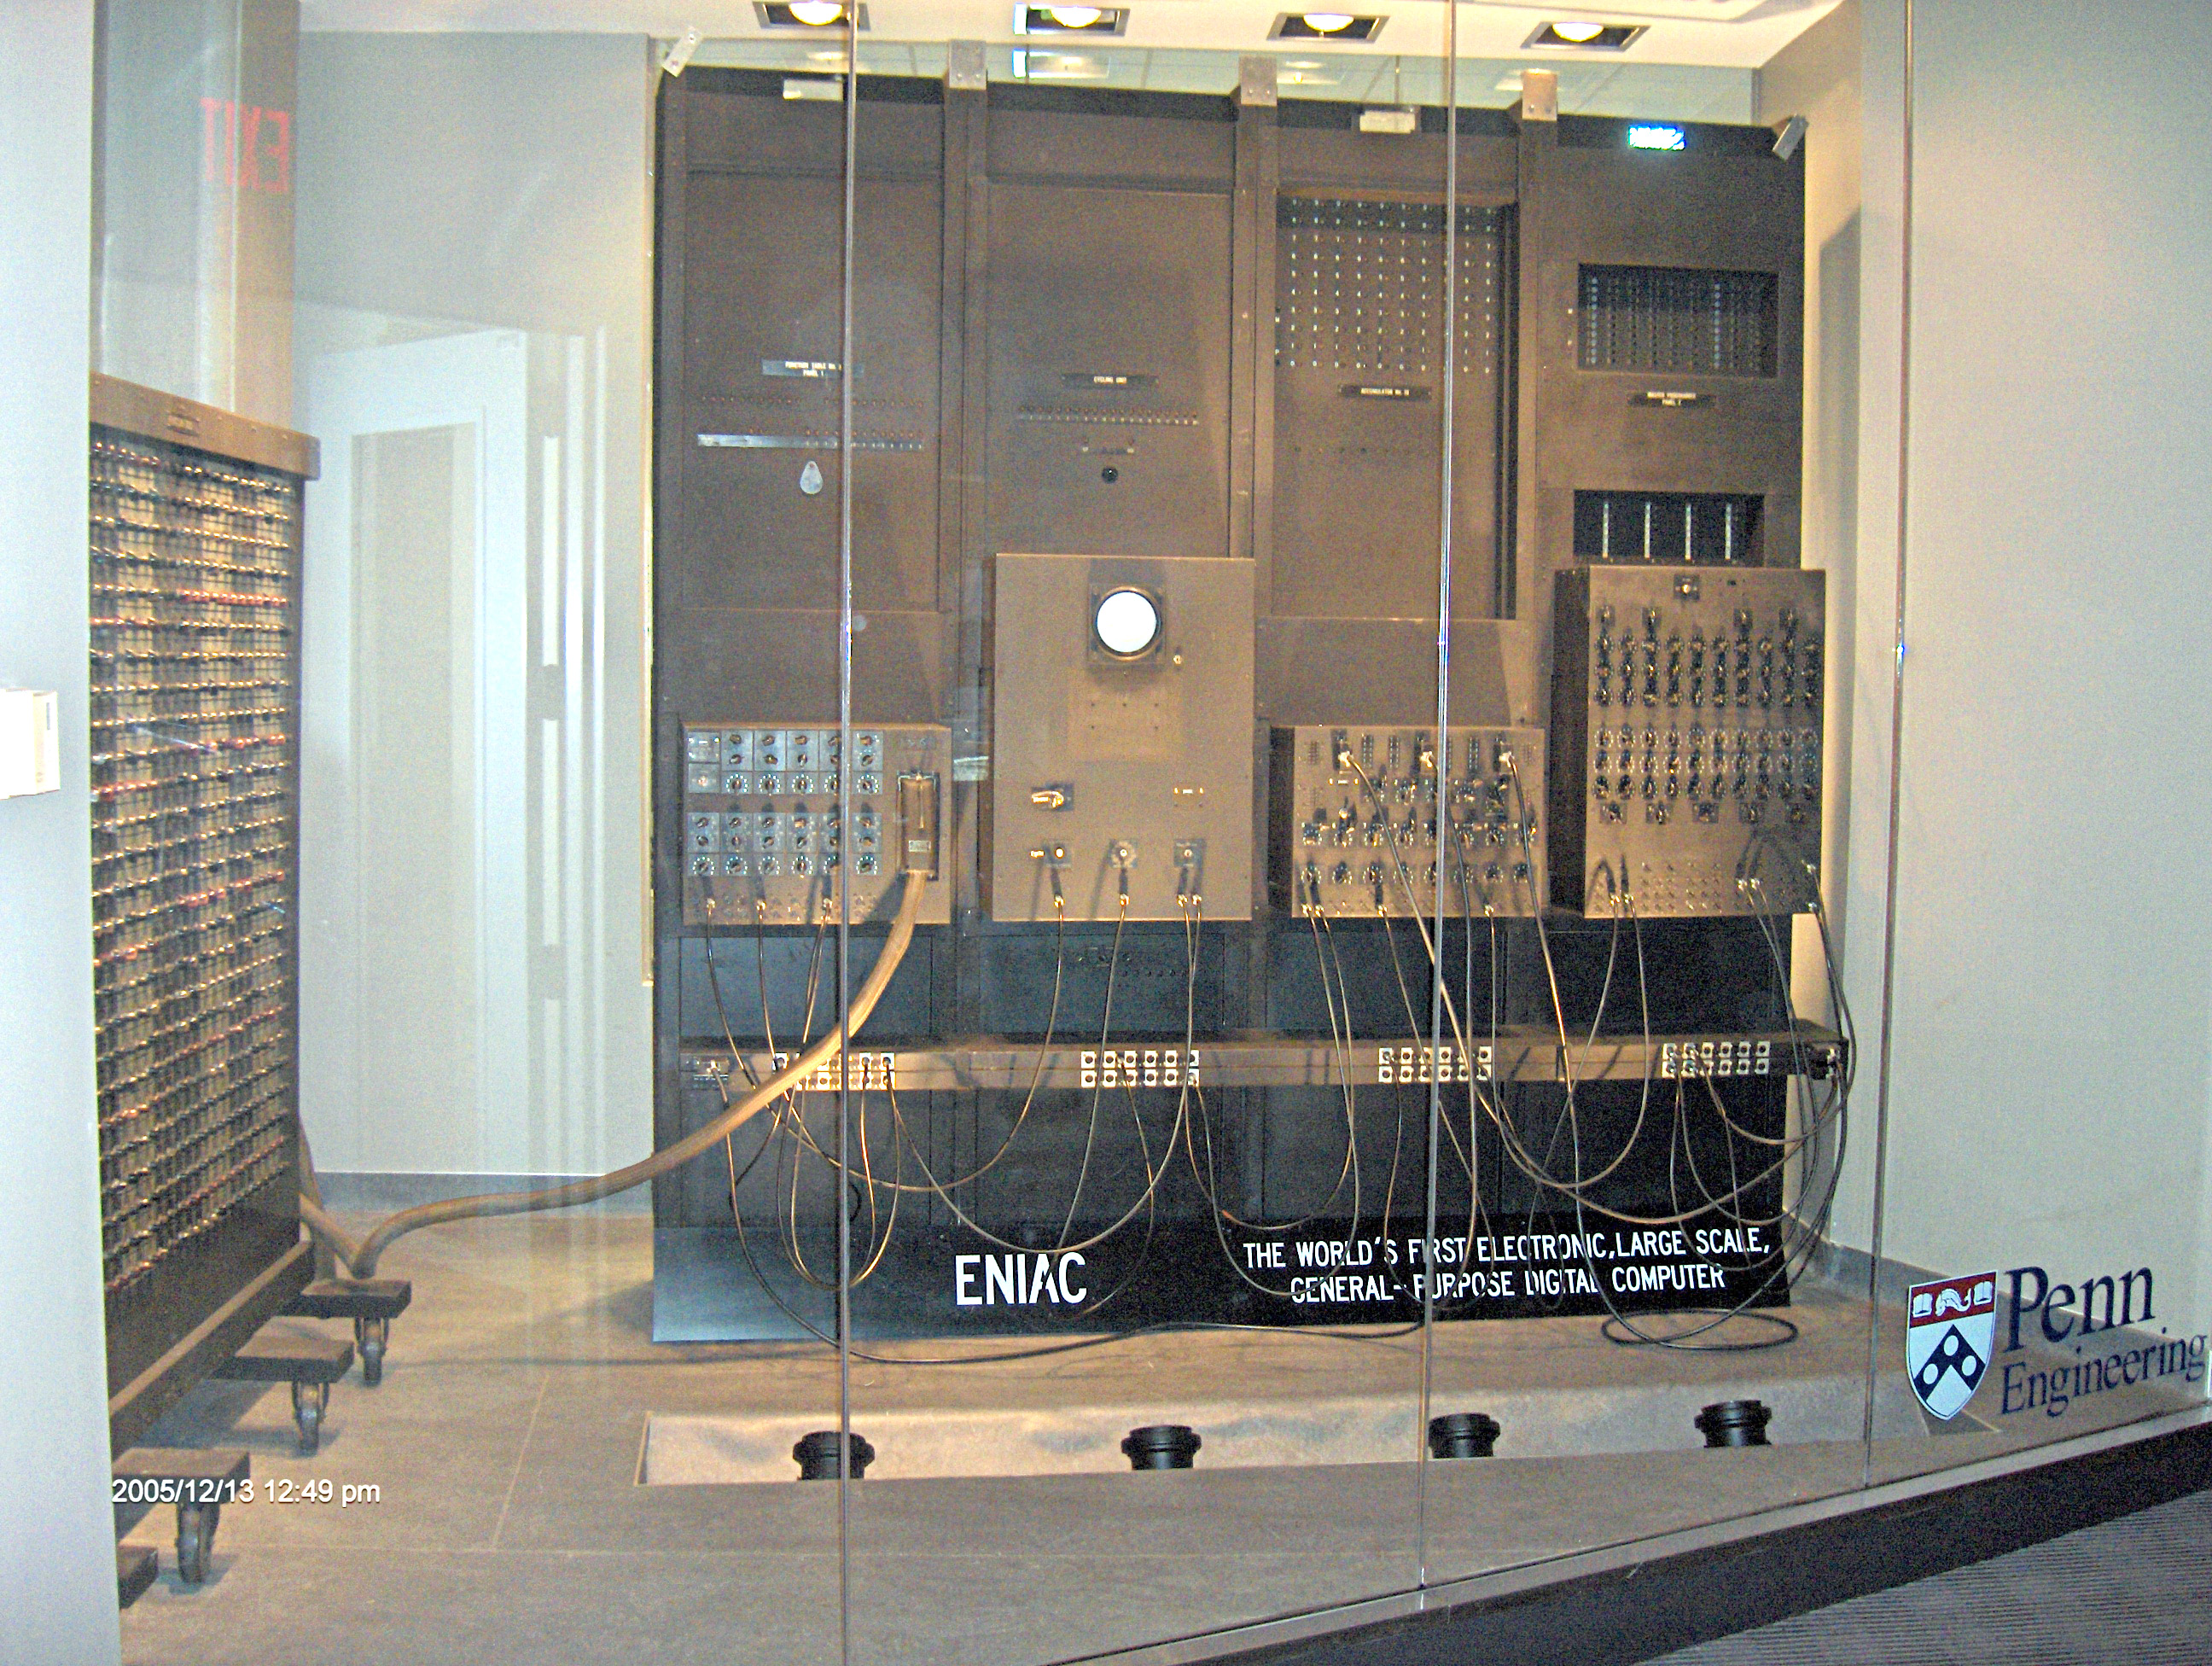
\includegraphics[width=0.4\textwidth]{compu}
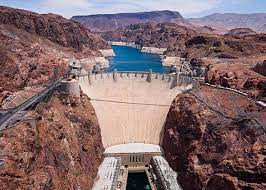
\includegraphics[width=0.4\textwidth]{hoov}
\end{center}
\end{frame}

\begin{frame}{En la actualidad}
\vspace{-0.4cm}
\begin{exampleblock}{}
\begin{itemize}
\item Modelos de predicción hidrológica y calidad de agua
\item Modelos de circulación global y oceánica a alta resolución
\item Optimización en el diseño de estructuras y sistemas de regadío y distribución
\end{itemize}
\end{exampleblock}
\begin{center}
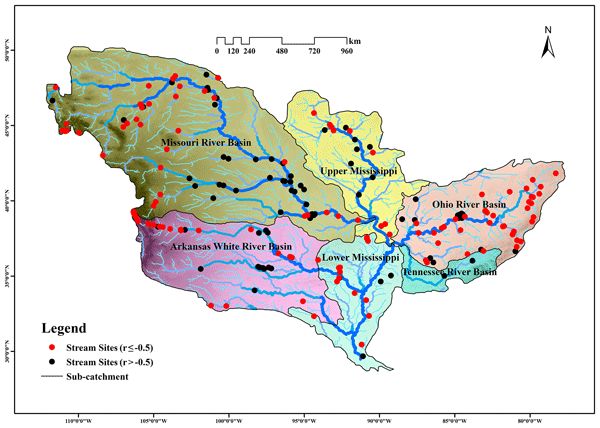
\includegraphics[width=0.4\textwidth]{rivba}
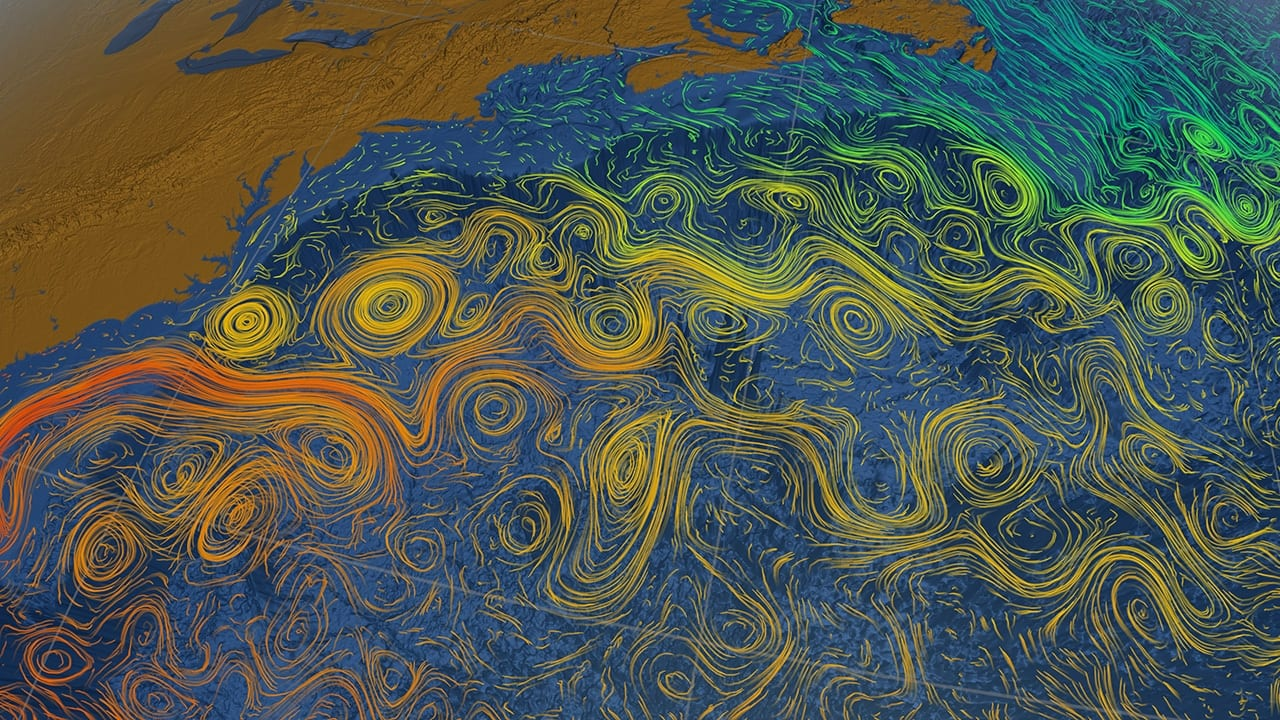
\includegraphics[width=0.4\textwidth]{oceanc}
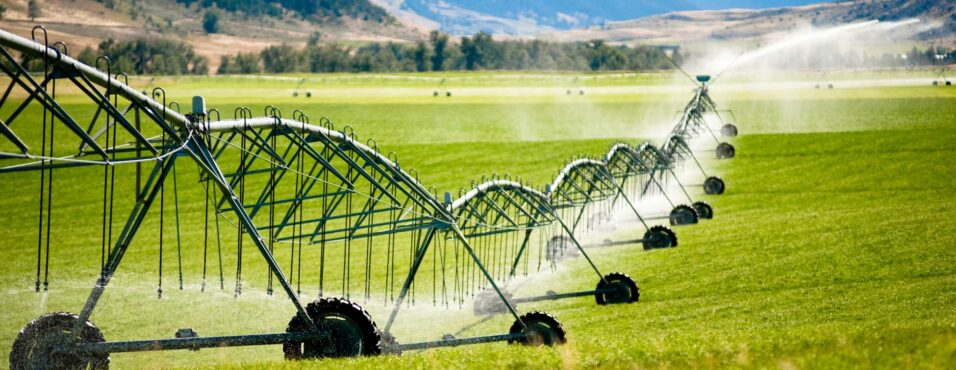
\includegraphics[width=0.4\textwidth]{irriga}
\end{center}
\end{frame}

\end{document}

